\documentclass[a4paper,12pt]{article}
\renewcommand{\familydefault}{\sfdefault}


%                   %
% Package importing %
%                   %

% Images, wraping
\usepackage{graphicx}
\usepackage{wrapfig}
\usepackage{float}

% Allow more floats per page
\setcounter{topnumber}{8}
\setcounter{bottomnumber}{8}
\setcounter{totalnumber}{8}

% Doc margins
\usepackage[left = 50pt, right = 50pt, top = 60pt, bottom = 60pt]{geometry}

% Line spacing
\usepackage[utf8]{inputenc}
\usepackage[english]{babel}

\setlength{\parindent}{0pt}

% Hyperlinks
\usepackage{hyperref}
\hypersetup {
	colorlinks = true,
	linkcolor = cyan,
	urlcolor = cyan,
}

% C# Code highlight
\usepackage{listings}
\usepackage{xcolor}
\usepackage{courier}
\lstset{basicstyle=\ttfamily,breaklines=true}
\lstset{framextopmargin=50pt,frame=bottomline}
\lstdefinestyle{sharpc}{
	language=[Sharp]C, 
	numbers=left,
	frame=l,
	numbersep=10pt,
	tabsize=2,
	rulecolor=\color{blue!80!black},
}
\lstset{style=sharpc}
 
 
% Start of document
\begin{document}


% Title
\title{Unity Tool: Dialogue Editor\vspace{-50pt}}
\date{}
\maketitle

\begin{figure}[ht]
\centering
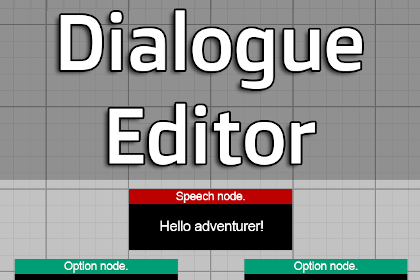
\includegraphics[width=250pt, keepaspectratio]{img/CardImage.png}
\end{figure}




% Links
\section{Links}
\begin{itemize}
\setlength\itemsep{1pt}
	\item \href{https://assetstore.unity.com/packages/tools/utilities/dialogue-editor-168329}{Asset store}
	\item \href{https://josephbarber96.github.io/dialogueeditor.html}{Online documentation}
	\item \href{https://www.youtube.com/playlist?list=PLfRF6lnXtGqjrhzyQhidqMD-shMHGReXi}{Video Tutorial Playlist}
\end{itemize}




% Sections
\section{Written Tutorial}
\begin{itemize}
\setlength\itemsep{1pt}
	\item \hyperlink{_whatis}{What is Dialogue Editor?}
	\item \hyperlink{_editorwindow}{Editor Window}
	\item \hyperlink{_conversationmanager}{Conversation Manager UI Prefab}
	\item \hyperlink{_triggering}{Triggering a conversation}
	\item \hyperlink{_custominput}{Custom Input}
	\item \hyperlink{_callbacks}{Callbacks}
	\item \hyperlink{_datastructure}{Conversation Datastructure}
\end{itemize}




% What is Dialogue Editor
\hypertarget{_whatis}{}
\section{What is Dialogue Editor?}
Dialogue Editor is a Unity tool that allows you to quickly and easily add conversations into your game.
\newline
The tool comes with an editor window that allows you to create and edit conversations.
\newline
This tool also comes with a pre-made, customisable UI prefab so that no UI programming is required. However, if you are comfortable with programming and wish to create your own UI implementation, each conversation can be accessed as a simple data structure.
\newpage




% Editor Window
\hypertarget{_editorwindow}{}
\section{Editor Window}

\subsection{Intro}
Conversations are made up of Speech nodes and Option nodes. Speech nodes represent something a character will say, and Option nodes represent the options available to the player. The connections between these nodes show the flow of the conversation. 

\begin{figure}[ht]
\centering
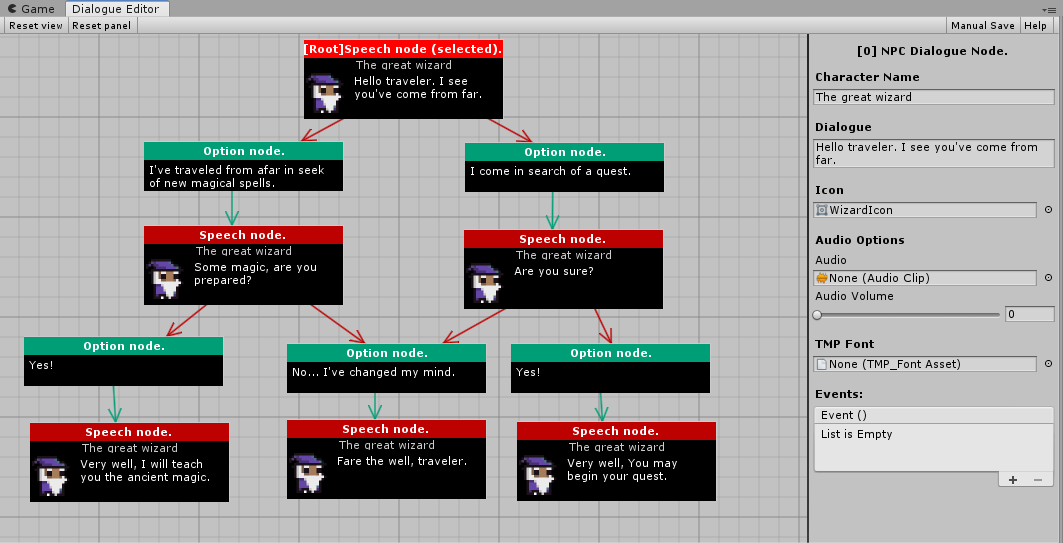
\includegraphics[width=0.8\textwidth, keepaspectratio]{img/EditorWindowFullConversation.png}
\end{figure}


\subsection{Creating a Conversation Object}
In order to create a conversation, create a new GameObject and add the script NPCConversation. 

\begin{figure}[ht]
\centering
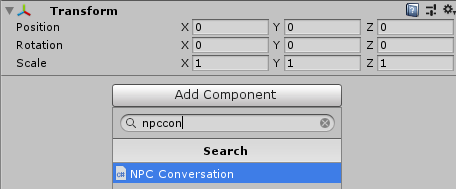
\includegraphics[width=300pt, keepaspectratio]{img/AddNpcConversation.png}
\end{figure}



\subsection{Opening the Editor Window}
In order to open the Editor Window, select Window $\rightarrow$ DialogueEditor. Select a conversation in the hierarchy in order to edit the conversation in the editor window.

\begin{figure}[h]
\centering
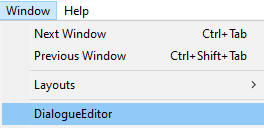
\includegraphics[width=200pt, keepaspectratio]{img/OpenEditorWindow.png}
\end{figure}

\newpage

\subsection{Speech Nodes}
When you create a new conversation, it will contain a single speech node - this is the beginning of the conversation. 
\newline
Click on a speech node to edit it. A speech node has the following variables:
\bigskip

% MINI PAGE - List

\begin{minipage}[c]{0.45\textwidth}
\begin{itemize}
\setlength\itemsep{1pt}
	\item \textbf{Character Name}: This is the name of the character who is speaking.
	\item \textbf{Dialogue}: This is the speech for the node.
	\item \textbf{Automatically Advance}: This option is available if a speech node leads onto another speech node, or nothing. When this option is selected, the dialogue will automatically continue without the user needing to click anything.
	% sub-list
	\begin{itemize}
		\item \textbf{Display Continue Options}: Should the "Continue" / "End" options still display?
		\item \textbf{Dialogue Time}: How long to wait before the dialogue automatically advances.
	\end{itemize}
	\item \textbf{Icon}: This is the icon of the NPC that will appear next to the speech.
	\item \textbf{Audio}: This is an optional variable, you can play audio with this speech.
	\item \textbf{TMPFont}: This is the TextMeshPro font for this speech. You are able to set fonts on a node-by-node basis.
	\item \textbf{Events}: These are Unity Events that will run when this speech node in a conversation is played.
\end{itemize}
\end{minipage}
\hfill
% MINI PAGE - image
\begin{minipage}[c]{0.45\textwidth}
\centering
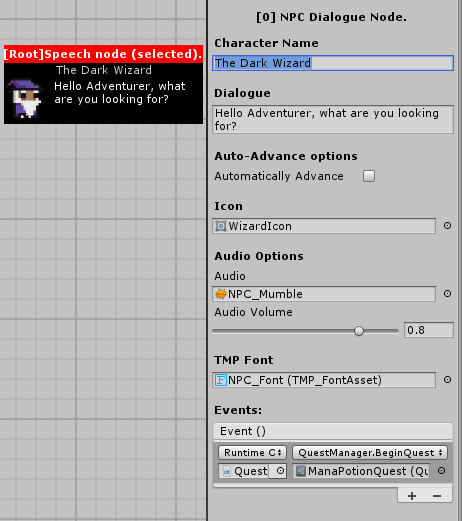
\includegraphics[width=\linewidth]{img/SpeechNode.png}
\end{minipage}

\bigskip

\subsection{Option Nodes}
An Option Node represents an option that a user can select.
\newline
Click on an option node to edit it. An option node has the following variables:

\begin{itemize}
\setlength\itemsep{1pt}
	\item \textbf{Option text}: This is the text for the option.
	\item \textbf{TMP Font}: This is the TextMeshPro font that the option text will use.
\end{itemize}

\newpage

\subsection{Creating Nodes}

To make a new node, right-click on an existing node. Select either "Create Speech" or "Create Option". Then, left-click somewhere to place the node.

\bigskip

\begin{minipage}[c]{0.45\textwidth}
\centering
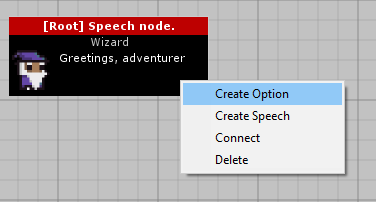
\includegraphics[width=225pt, keepaspectratio]{img/CreateNode.png}
\end{minipage}
\hfill
\begin{minipage}[c]{0.45\textwidth}
\centering
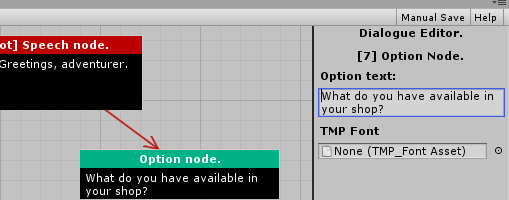
\includegraphics[width=225pt, keepaspectratio]{img/PlaceNode.png}
\end{minipage}

\subsection{Connecting Nodes}

To connect two existing nodes, right-click on a node and click "Connect". Then, left-click on the node you wish to connect it to. 

Speech nodes can be connected to option nodes, or other speech nodes. 

\begin{itemize}
\setlength\itemsep{1pt}
	\item If a speech node connects to option nodes, these options will appear for the player.
	\item If a speech node connects to another speech node, the following speech node will occur afterwards.
	\item If a speech node is connected to nothing, it marks the end of the conversation.
\end{itemize}
\bigbreak

Option nodes can only be connected to speech nodes.
\begin{itemize}
\setlength\itemsep{1pt}
	\item If an option node connects to a speech node, the following speech node will occur after selecting the option.
	\item If an option node is connected to nothing, the conversation will end after selecting the option.	
\end{itemize}

\subsection{Deleting Nodes and Connections}
Unwanted connections between nodes can be deleted by right-clicking on the arrow and clicking "Delete this connection"
\newline
Likewise, unwanted nodes can also be deleted by right-clicking on the node and clicking "Delete this node". Deleting a node will also delete any connection to and from this node.
\bigskip 

\begin{minipage}[c]{0.45\textwidth}
\centering
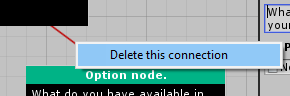
\includegraphics[keepaspectratio]{img/DeleteConnection.png}
\end{minipage}
\hfill
\begin{minipage}[c]{0.45\textwidth}
\centering
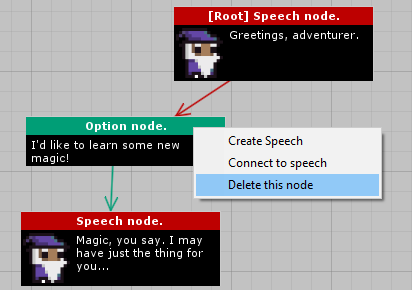
\includegraphics[width=200pt, keepaspectratio]{img/DeleteNode.png}
\end{minipage}

\newpage



\subsection{Parameters and Conditions}
A conversation can have parameters. These will have a name and a value; the value can be updated. A connection between nodes can have conditions, so that the connection will only be valid if the conditions are met. Conditions require a parameter value to meet certain requirements.

\subsubsection{Adding Parameters}
By having nothing in the conversation selected, you can see the Parameters. You can add Int and Bool parameters by clicking the Add Int and Add Bool buttons respectively. You can re-name these parameters and give them a default value. 

\begin{figure}[h]
\centering
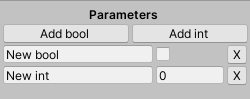
\includegraphics[keepaspectratio]{img/Parameters.png}
\end{figure}

\subsubsection{Adding Conditions}
By clicking on a connection, you can set conditions. This connection will only be valid if the conditions are all met. This allows you to create scenarios in which specific options or pieces of dialogue will only be shown to players who meet the requirements. 

\begin{figure}[h]
\centering
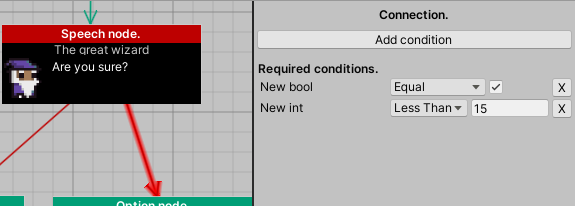
\includegraphics[keepaspectratio]{img/ConnectionConditions.png}
\end{figure}
\newpage

\subsubsection{Setting Parameter Values}

\textbf{By Action}
\bigskip

By clicking on a Speech node or Option node, you can click "Add Parameter Action". This allows you to set the value of any parameters when either the speech is activated, or the option is selected.

\begin{figure}[hb]
\centering
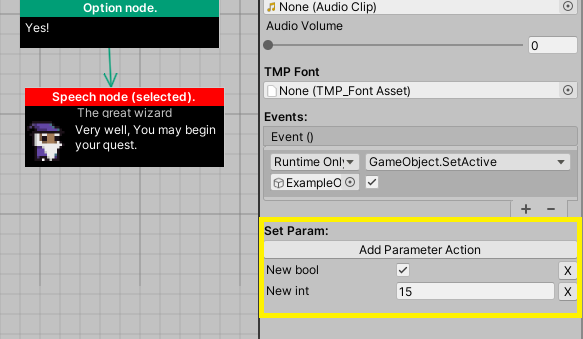
\includegraphics[keepaspectratio]{img/SetParam.png}
\end{figure}
\bigskip

\textbf{By Code}
\bigskip

You can also get and set the values of Parameters at run time by code. You can do this by calling the appropriate functions on the ConversationManager.
\newline

Note: You will need to add the "DialogueEditor" namespace to your script. This can be done by adding the following line at the top:
\bigskip

\begin{lstlisting}
using DialogueEditor;
\end{lstlisting}
\bigskip

You can call the following functions to get/set the parameter values:
\bigskip

\begin{lstlisting}
// Set
ConversationManager.Instance.SetBool("BoolName", true);
ConversationManager.Instance.SetInt("IntName", 1);

// Get
bool bVal = ConversationManager.Instance.GetBool("BoolName");
int iVal = ConversationManager.Instance.GetInt("IntName");
\end{lstlisting}
\bigskip

\newpage




% Conversation Manager 
\hypertarget{_conversationmanager}{}
\section{Conversation Manager}
A pre-made, customisable UI prefab is provided. The ConversationManager contains all of the UI, therefore, to add it into the scene, you drag it as a child of a UI Canvas. 
\newline
\newline
When you drag the ConversationMaanager prefab into your scene, if you do not have TextMeshPro in the Unity project, it will prompt you to Import TMP Essentials. After importing, please delete the ConversationManager from the hierarchy, and then re-add it back into the hierarchy, so that it can render correctly with TMP.
\newline
\begin{figure}[h]
\centering
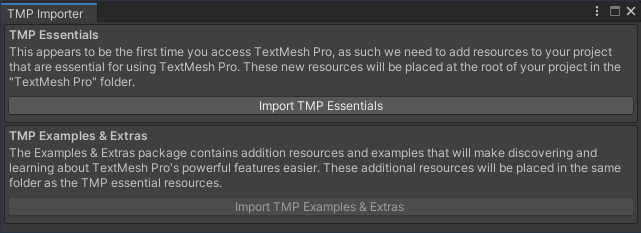
\includegraphics[width=400pt, keepaspectratio]{img/ImportTMPEssentials.png}
\end{figure}
\newline
Recommended canvas settings:
\begin{itemize}
\setlength\itemsep{1pt}
	\item \textbf{Canvas - Render Mode}: Screen Space - Overlay
	\item \textbf{Canvas Scaler - UI Scale Mode}: Scale with Screen Size
\end{itemize}

\begin{figure}[h]
\centering
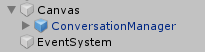
\includegraphics[keepaspectratio]{img/CanvasInHierarchy.png}
\end{figure}

\begin{figure}[h]
\centering
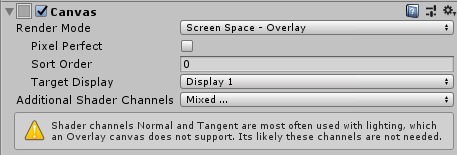
\includegraphics[width=250pt, keepaspectratio]{img/CanvasComponent.png}
\end{figure}


\begin{figure}[h]
\centering
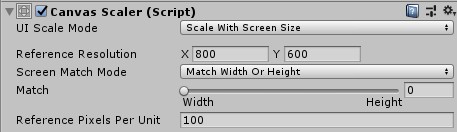
\includegraphics[width=250pt, keepaspectratio]{img/CanvasScalarComponent.png}
\end{figure}

\newpage

The ConversationManager provides options for the Background image of the Dialogue box and the Options box. These images can be optionally 9-sliced images. A preview render is displayed above the options. You can also select text-scrolling options.

\begin{figure}[h]
\centering
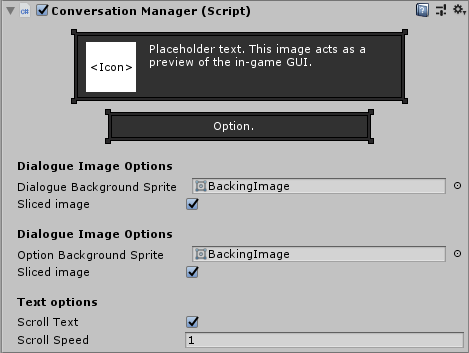
\includegraphics[width=300pt, keepaspectratio]{img/ConversationManager.png}
\end{figure}

\newpage




% Triggering a conversation
\hypertarget{_triggering}{}
\section{Triggering a Conversation}

If you are using the ConversationManager UI Prefab, conversations can be triggered by calling a single function, and passing through an NPCConversation variable:
\bigskip

\begin{lstlisting}
ConversationManager.Instance.StartConversation(/*NPCConversation*/);
\end{lstlisting}
\bigskip

Note: You will need to add the "DialogueEditor" namespace to your script. This can be done by adding the following line at the top:
\bigskip

\begin{lstlisting}
using DialogueEditor;
\end{lstlisting}
\bigskip

Here is some example code, which shows a very basic NPC class which begins a conversation when the NPC is clicked on:
\bigskip

\begin{lstlisting}
using UnityEngine;
using DialogueEditor;

public class NPC : MonoBehaviour
{
	// NPCConversation Variable (assigned in Inspector)
	public NPCConversation Conversation;

	private void OnMouseOver()
	{
		if (Input.GetMouseButtonDown(0))
		{
			ConversationManager.Instance.StartConversation(Conversation);
		}
	}
}
\end{lstlisting}
\bigskip


There are also a number of additional Properties and Functions available to you:
\bigskip

\begin{lstlisting}
// Is a conversation currently happening?
ConversationManager.Instance.IsConversationActive;

// The current conversation (null if no conversation active).
ConversationManager.Instance.CurrentConversation;

// End a conversation early (e.g. player walks off).
ConversationManager.Instance.EndConversation();
\end{lstlisting}


\newpage




% Custom Input
\hypertarget{_custominput}{}
\section{Custom Input}
Dialogue Editor provides some basic functions which allows you to interact with the Conversation UI. This enables you to support any input method that your game supports, such as Keyboard + Mouse or a Controller.
\newline
Three basic functions allow you to cycle to the next or previous option, and to press the currently selected option:
\bigskip

\begin{lstlisting}
// Cycle to the previous option
ConversationManager.Instance.SelectPreviousOption();
// Cycle to the next option
ConversationManager.Instance.SelectNextOption();
// Press the currently selected option
ConversationManager.Instance.PressSelectedOption();
\end{lstlisting}
\bigskip

Here is some example code which shows keyboard support for the Conversation UI:
\bigskip

\begin{lstlisting}
Using UnityEngine;
Using DialogueEditor;

public class ExampleInputManager : MonoBehaviour
{
	private void Update()	
	{
		if (ConversationManager.Instance != null)
		{
			if (ConversationManager.Instance.IsConversationActive)
			{
				if (Input.GetKeyDown(KeyCode.UpArrow))
					ConversationManager.Instance.SelectPreviousOption();
					    
				else if (Input.GetKeyDown(KeyCode.DownArrow))
					ConversationManager.Instance.SelectNextOption();
					
				else if (Input.GetKeyDown(KeyCode.F))
					ConversationManager.Instance.PressSelectedOption();
			}
		}
	}
}
\end{lstlisting}
\bigskip

There is also an option on the Conversation Manager prefab which allows you to choose whether or not mouse interaction should be enabled.

\begin{figure}[ht]
\centering
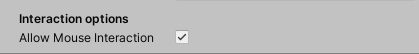
\includegraphics[keepaspectratio]{img/AllowMouseInteraction.png}
\end{figure}

\newpage





% Callbacks
\hypertarget{_callbacks}{}
\section{Callbacks}

If you are using the ConversationManager UI Prefab, there are two callbacks available to you which are invoked when a conversation starts and ends, respectively.
\bigskip

\begin{lstlisting}
DialogueEditor.ConversationManager.OnConversationStarted
DialogueEditor.ConversationManager.OnConversationEnded
\end{lstlisting}
\bigskip

Note: You will need to add the "DialogueEditor" namespace to your script. This can be done by adding the following line at the top:
\bigskip

\begin{lstlisting}
using DialogueEditor;
\end{lstlisting}
\bigskip

Example use-case:
\bigskip

\begin{lstlisting}
using UnityEngine;
using DialogueEditor;

public class ExampleClass : MonoBehaviour
{
	private void OnEnable()
	{
		ConversationManager.OnConversationStarted += ConversationStart;
		ConversationManager.OnConversationEnded += ConversationEnd;
	}
	
	private void OnDisable()
	{
		ConversationManager.OnConversationStarted -= ConversationStart;
		ConversationManager.OnConversationEnded -= ConversationEnd;
	}
	
	private void ConversationStart()
	{
		Debug.Log("A conversation has began.");
	}
	
	private void ConversationEnd()
	{
		Debug.Log("A conversation has ended.");
	}
}
\end{lstlisting}

\newpage

% Datastructure
\hypertarget{_datastructure}{}
\section{Conversation Datastructure}

This section contains information for people who want to code their own custom UI implementation. If you want to use the pre-made UI that comes with the tool, this section can be ignored.

\subsection{Deserialising}
Note: You will need to add the "DialogueEditor" namespace to your script. This can be done by adding the following line at the top:
\bigskip

\begin{lstlisting}
using DialogueEditor;
\end{lstlisting}
\bigskip

In order to deserialize the conversation, NPCConversation contains a function for doing so: this returns an object of type "Conversation":
\bigskip

\begin{lstlisting}
NPCConversation NPCConv;
Conversation conversation = NPCConv.Deserialize();
\end{lstlisting}
\bigskip

Here are the classes that you will need to be concerned with when creating your custom UI implementation: 


\subsection{Converstion}
An NPCConversation deserializes into a tree-like data structure. Deserialising will return you an object of type "Conversation". A Conversation object contains a SpeechNode; the root of the conversation - from here, the nodes are connected in a tree-like pattern. The Conversation object also contains all the Parameters of a conversation, and functionality to Set and Get parameter values. 
\begin{lstlisting}
public class Conversation
{
	public Conversation()
	{
		Parameters = new List<Parameter>();
	}

	/// <summary> The start of the conversation </summary>
	public SpeechNode Root;

	/// <summary> The parameters of this conversation, and their values </summary>
	public List<Parameter> Parameters;

	/* Method implementation and private methods ommitted */

	public void SetInt(string paramName, int value, out eParamStatus status);
	public void SetBool(string paramName, bool value, out eParamStatus status)
	public int GetInt(string paramName, out eParamStatus status);	
	public bool GetBool(string paramName, out eParamStatus status);
}
\end{lstlisting}
\newpage


\subsection{ConversationNode}
A ConversationNode is either a SpeechNode or an OptionNode. A ConversationNode contains all data about that node (E.g. Dialogue text, TMP Font, UnityEvent, Param Actions, etc) as well as all Connections that node has. 
\begin{lstlisting}
public abstract class ConversationNode
{
	public enum eNodeType
	{
		Speech,
		Option
	}

	public ConversationNode()
	{
		Connections = new List<Connection>();
		ParamActions = new List<SetParamAction>();
	}

	public abstract eNodeType NodeType { get; }
	public Connection.eConnectionType ConnectionType { get { /* Ommited */ } }

	/// <summary> The body text of the node. </summary>
	public string Text;

	/// <summary> The child connections this node has. </summary>
	public List<Connection> Connections;

	/// <summary> This nodes parameter actions. </summary>
	public List<SetParamAction> ParamActions;

	/// <summary> The Text Mesh Pro FontAsset for the text of this node. </summary>
	public TMPro.TMP_FontAsset TMPFont;
}


public class SpeechNode : ConversationNode
{
	public override eNodeType NodeType { get { return eNodeType.Speech; } }

	/// <summary> The name of the NPC who is speaking. </summary>
	public string Name;

	/// <summary> Should this speech node go onto the next one automatically? </summary>
	public bool AutomaticallyAdvance;

	/// <summary> Should this speech node, althought auto-advance, also display a "continue" or "end" option, for users to click through quicker? </summary>
	public bool AutoAdvanceShouldDisplayOption;

	/// <summary> If AutomaticallyAdvance==True, how long should this speech node display before going onto the next one? </summary>
	public float TimeUntilAdvance;

	/// <summary> The Icon of the speaking NPC </summary>
	public Sprite Icon;

	public AudioClip Audio;
	public float Volume;

	/// <summary> UnityEvent, to betriggered when this Node starts. </summary>
	public UnityEngine.Events.UnityEvent Event;
}


public class OptionNode : ConversationNode
{
	public override eNodeType NodeType { get { return eNodeType.Option; } }
}
\end{lstlisting}
\newpage

\subsection{Connection}
Each ConversationNode has a list of 0 or more Connections. A Connection contains a SpeechNode or OptionNode, as well as  list of Conditions. 
\begin{lstlisting}
public abstract class Connection
{
	public enum eConnectionType
	{
		None,
		Speech,
		Option
	}

	public Connection()
	{
		Conditions = new List<Condition>();
	}

	public abstract eConnectionType ConnectionType { get; }

	public List<Condition> Conditions;
}

public class SpeechConnection : Connection
{
	public SpeechConnection(SpeechNode node)
	{
		SpeechNode = node;
	}

	public override eConnectionType ConnectionType { get { return eConnectionType.Speech; } }

	public SpeechNode SpeechNode;
}

public class OptionConnection : Connection
{
	public OptionConnection(OptionNode node)
	{
		OptionNode = node;
	}

	public override eConnectionType ConnectionType { get { return eConnectionType.Option; } }

	public OptionNode OptionNode;
}
\end{lstlisting}
\newpage


\subsection{Condition}
Each Connection has a list of 0 or more Conditions. Each Condition contains the name of the parameter, a CheckType (e.g. EqualTo, GreaterThan) and the RequiredValue.
\begin{lstlisting}
public abstract class Condition
{
	public enum eConditionType
	{
		IntCondition,
		BoolCondition
	}

	public abstract eConditionType ConditionType { get; }

	public string ParameterName;
}

public class IntCondition : Condition
{
	public enum eCheckType
	{
		equal,
		lessThan,
		greaterThan
	}

	public override eConditionType ConditionType { get { return eConditionType.IntCondition; } }

	public eCheckType CheckType;
	public int RequiredValue;
}

public class BoolCondition : Condition
{
	public enum eCheckType
	{
		equal,
		notEqual
	}

	public override eConditionType ConditionType { get { return eConditionType.BoolCondition; } }

	public eCheckType CheckType;
	public bool RequiredValue;
}
\end{lstlisting}
\newpage


\subsection{Parameter}
Each Conversation can have unique Parameters. Each Parameter has a Name and a Value. These Parameters are used to create Conditions for Connections
\begin{lstlisting}
public abstract class Parameter
{
	public Parameter(string name)
	{
		ParameterName = name;
	}

	public string ParameterName;
}

public class BoolParameter : Parameter
{
	public BoolParameter(string name, bool defaultValue) : base(name)
	{
		BoolValue = defaultValue;
	}

	public bool BoolValue;
}

public class IntParameter : Parameter
{
	public IntParameter(string name, int defalutValue) : base(name)
	{
		IntValue = defalutValue;
	}

	public int IntValue;
}
\end{lstlisting}
\newpage


\subsection{SetParamAction}
The SetParamAction class defines a Parameter Name and a Value. Each ConversationNode has a list of 0 or more ParamActions - when this ConversationNode is either played (Speech node) or selected by the user (Option node) the ParamActions should be executed - the parameters defined by ParameterName should be set to the specified Value.
\begin{lstlisting}
public abstract class SetParamAction
{
	public enum eParamActionType
	{
		Int,
		Bool
	}

	public abstract eParamActionType ParamActionType { get; }

	public string ParameterName;
}

public class SetIntParamAction : SetParamAction
{
	public override eParamActionType ParamActionType { get { return eParamActionType.Int; } }

	public int Value;
}

public class SetBoolParamAction : SetParamAction
{
	public override eParamActionType ParamActionType { get { return eParamActionType.Bool; } }

	public bool Value;
}
\end{lstlisting}



\newpage
\end{document}